\section{A methodology for the study of latency-sensitive applications in Edge Computing}\label{summary:methodology}

This thesis makes a contribution to the field of Edge Computing by investigating the applications of a methodology for the study of latency-sensitive applications deployed on Edge infrastructure.
These applications, such as \gls{WCA} and \glspl{NCS}, are challenging to study and scale due to their cyber-physical nature, complexity, and requirements for low latency and high reliability.

The main focus of this thesis is to enhance the accuracy and realism of results related to Edge infrastructure, particularly in regard to the network.
The proposed methodology aims to provide a more comprehensive and realistic assessment of the performance of these latency-sensitive applications, allowing for a better understanding of the strengths and limitations of Edge Computing in this context.
Our results will contribute to the development of new techniques and approaches for improving the performance and reliability of Edge Computing systems.

\begin{figure}
    \centering
    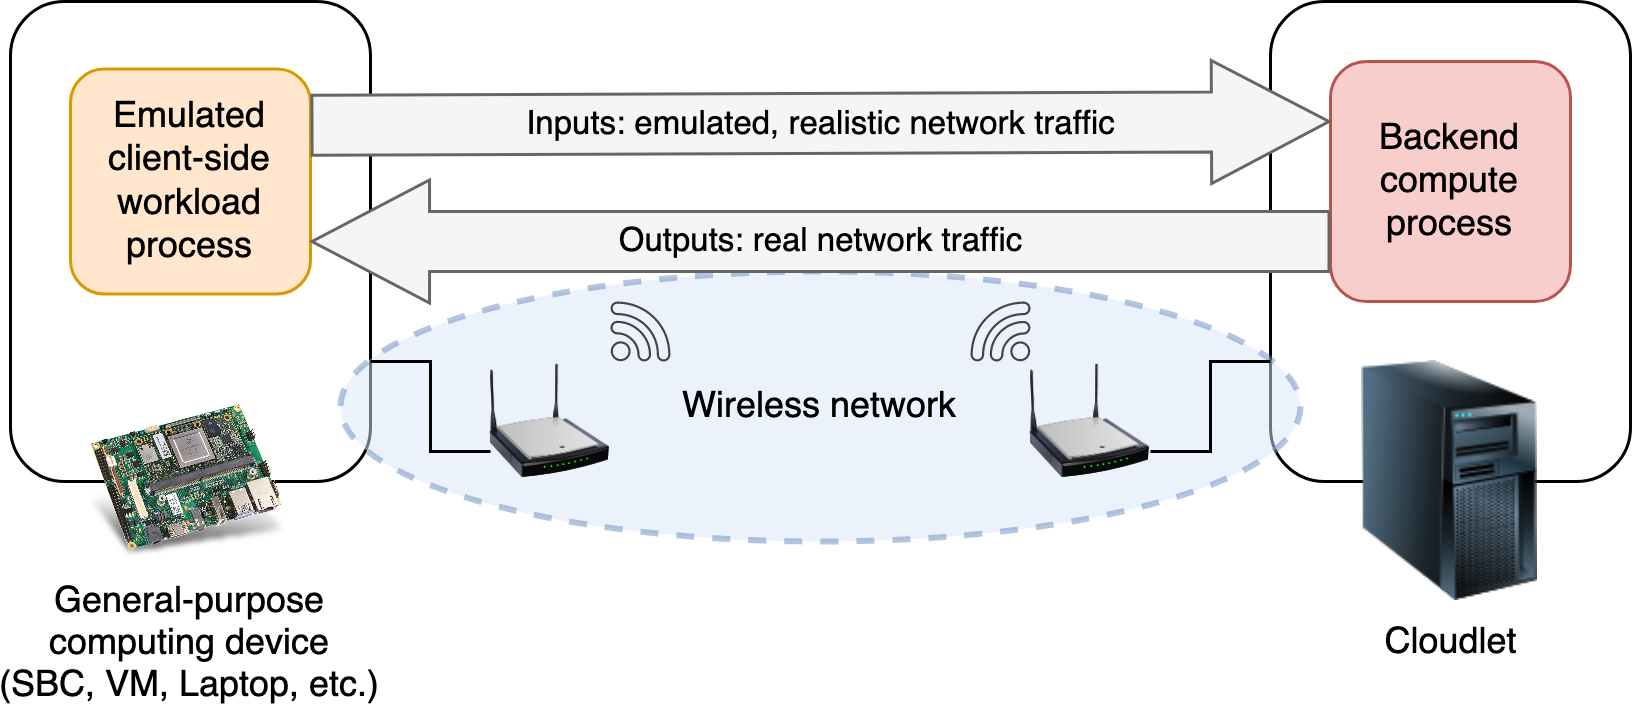
\includegraphics[width=.8\textwidth]{Figs/methodology}
    \caption{%
        Overview of the proposed methodology for the study of latency-sensitive systems on edge computing infrastructure.
        The  client side of the system is replaced with an emulation executed on a general-purpose computing device.
        The backend/server side of the system along with the network remain unchanged.
    }\label{fig:methodology}
\end{figure}

Our methodology is based on the emulation of target workloads on actual Edge infrastructure;
see \cref{fig:methodology}.
We replace the client side of the system with a realistic emulation of the desired behaviors;
this emulation is implemented in software deployed on \gls{COTS} general-purpose computing devices.
In our initial implementation, these correspond to low-cost, easily replaceable and scalable Raspberry Pi 4 Model B~\cite{raspberrypi} \glspl{SBC}.
We aim to maintain the backend software and hardware, as well as the network, unchanged with respect to the real-world deployment, in order to preserve as much realism as possible in the effects arising from the hardware and network.

As discussed in \cref{chap:relatedwork}, most research in this field falls into either simulated or fully-practical real-world approaches.
Our emulated methodology presents several advantages over these alternatives.
To begin with, and perhaps most importantly, it makes our approach portable and applicable to real edge computing deployments.
By limiting the emulation to the workload, our approach can be directly employed on pre-existing edge computing infrastructure in order to benchmark applications before they are deployed.
This makes our approach valuable to not only to the research community, but also to system designers and application developers.

In hand with the previous point, it allows for easier scaling compared to real-world studies.
The systems we target exhibit a centralized nature in which a potentially large number of clients offload computation to a single central compute node.
The client-side component of the applications of interest for this research is often complex to scale.
Consider a system owner interested in studying the performance of some edge computing setup for latency-sensitive applications.
In the case of interactive and immersive applications, scaling the number of human users is a significant challenge, as recruiting participants is an expensive and time-consuming endeavor.
Scaling applications involving \glspl{CPS} such as \glspl{NCS} can be prohibitively complex and expensive depending on the specific hardware involved.
In many cases, these systems are made-to-order, further increasing the cost as economies of scale cannot be employed.
On the other hand, a simulated approach requires modeling not only the application workload, but also the edge computing system and infrastructure.
Due to the intricate nature of contemporary cloud and edge computing setups, which frequently involve multiple tiers of proxies, load balancers, virtualized computing units, and network functions, the modeling of such systems can quickly become an overly complex endeavor.

Our approach circumvents both of these limitations.
Emulating the workload component reduces complexity by moving it into the software domain, allowing for easier scaling through the use of cheap, \gls{COTS} general-purpose hardware such as the aforementioned \glspl{SBC}.
Furthermore, it preserves the realism of effects stemming from the hardware and network.
Employing emulations allows our methodology to realize a more realistic testing environment than a simulated approach and can provide results that are closer to what would be seen in the real-world.
Of particular interest to us are effects due to network factors such as contention, congestion control, and medium access.
These effects are often of stochastic or chaotic natures, and are thus complex to capture in simulations.

Emulating the workload also provides improved repeatability and replicability.
Repeating a study becomes a matter of re-running the workload on the same testbed;
in turn, studies can be replicated simply by obtaining the same or equivalent software workload and deploying it on a comparable testbed.
These are complex tasks to accomplish in real-world approaches, particularly when dealing with humans.

Finally, our methodology improves extensibility significantly.
Replicating the methodology for other workloads simply requires developing a new piece of software to emulate the new workload.
This can further be simplified by employing software platforms for the emulation of categories of workloads, as well will discuss later on in this thesis.

\medskip
In the following subsections we will discuss two illustrative use-cases for our methodology; \acl{WCA} and \acl{NCS} research and benchmarking.
\Cref{summary:methodology:usecase_wca} discusses the application of our methodology to \gls{WCA}.
This work was originally published in \cref{paper:olguinmunoz2018demoscaling,paper:olguinmunoz2019edgedroid}.
Next, in \cref{summary:methodology:usecase_ncs} we expand this discussion to \glspl{NCS}, a discussion originally approached in \cref{paper:olguinmunoz2022cleave}.

\subsection{Use case: \acl{WCA}}\label{summary:methodology:usecase_wca}

\begin{figure}
    \centering
    \begin{subfigure}[b]{.45\textwidth}
        \centering
        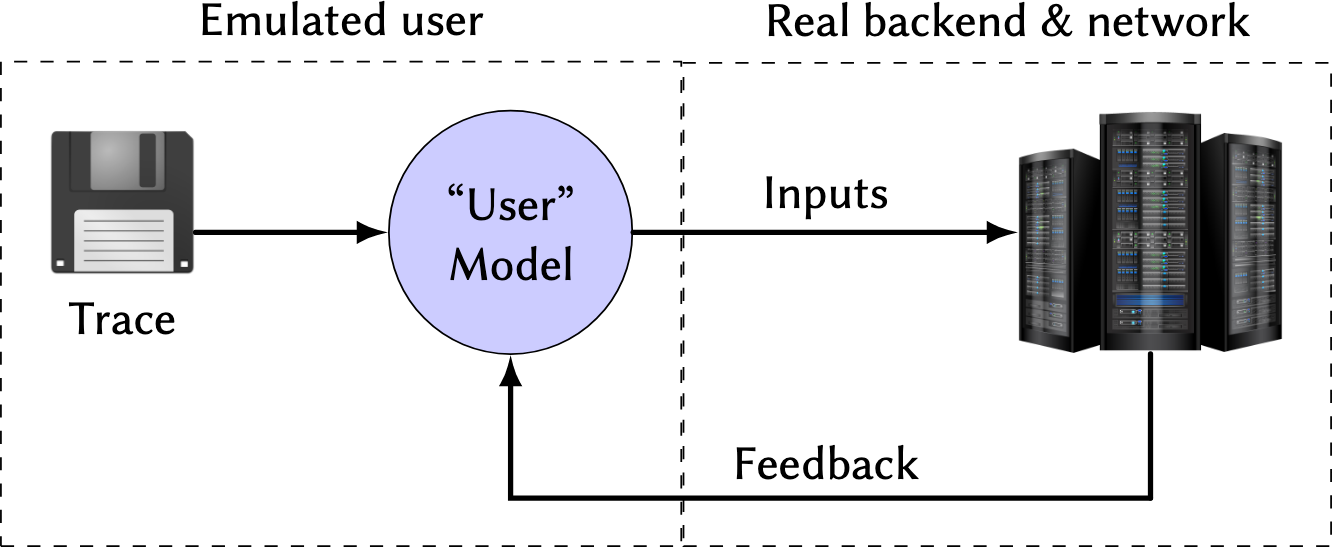
\includegraphics[width=\textwidth]{Figs/trace_edgedroid}
        \caption{%
            High level conceptual design of our methodology for \gls{WCA}.
            We replace the human by a trace-driven emulation.
            This allows us to maintain realism in inputs sent over the network to the compute process on the backend, while simplifying the design of the client software.
        }\label{fig:methodology:wca:conceptual}
    \end{subfigure}
    \hfill
    \begin{subfigure}[b]{.45\textwidth}
        \centering
        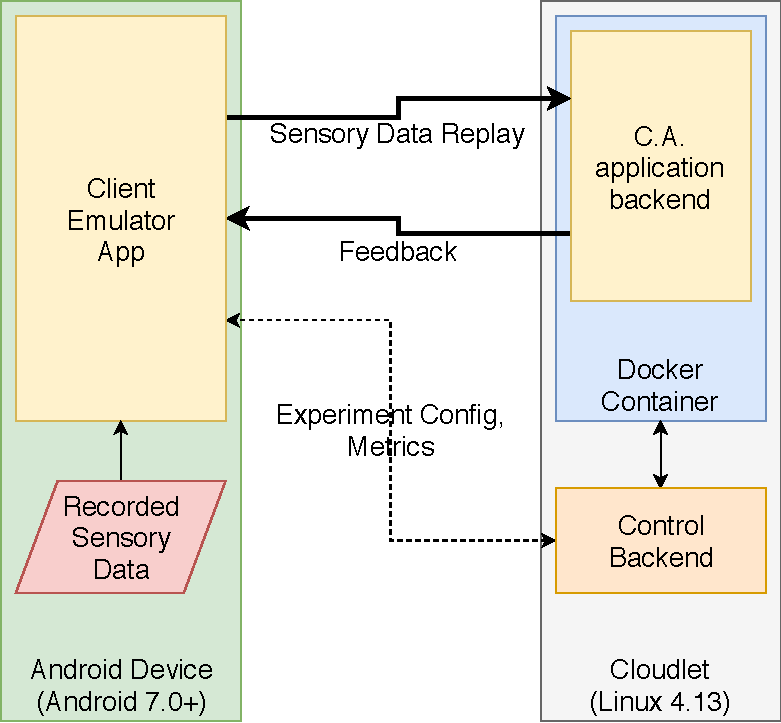
\includegraphics[width=\textwidth]{publications/2018DemoScalingOnTheEdge/img/TraceReplay_GenArch}
        \caption{%
            Architectural overview of the EdgeDroid \num{1.0} tool.
            The ``client emulator app'' implements the aforementioned user model together with the required networking functionality to connect to a \gls{WCA} backend running on a cloudlet.%
        }
    \end{subfigure}\\
    \medskip
    \begin{subfigure}[t]{\textwidth}
        \centering
        \adjustbox{scale=0.7}{
            \begin{tikzpicture}[align=center,
                node distance=.5cm and 1.5cm,
                every initial by arrow/.style={-{Latex[length=2mm]}}]
                % Place nodes
                \node [initial, state, minimum size=6em, initial text=] (play) {Play};
                \node [state, above right=of play, minimum size=6em] (change) {Change\\step};
                \node [state, below right=of play, minimum size=6em] (rewind) {Rewind};
                \node [state, accepting, above right=of rewind, minimum size=6em] (shutdown) {Shutdown};

                % Draw edges
                \path[draw, -{Latex[length=2mm]}]
                (play) edge [bend right=20] node[left] {Step done} (rewind)
                edge [bend left=20] node[left] {Got feedback\\(\emph{positive})} (change)
                edge [out=140,in=220,looseness=6] node[left] {Step\\not done} (play)

                (change) edge [bend left=20] node[right] {Step changed} (play)
                edge [bend left=20] node[right] {All steps done} (shutdown)

                (rewind) edge [bend right=20] node[right] {Rewound} (play)
                edge [bend right=20] node[right] {Too many rewinds} (shutdown);

            \end{tikzpicture}
        }
        \caption{State diagram of the user model governing the replay of the pre-recorded trace at runtime. This model approximates the behavior of an ``ideal'' human, one that is patient and makes no mistakes.}\label{fig:usermodel}
    \end{subfigure}
    \caption{%
        Overview of our first implementation of the methodology for \gls{WCA}.
        Figures originally published in \cref{paper:olguinmunoz2019edgedroid}.
    }
\end{figure}

We first introduce our methodology and its applicability to \gls{WCA} in \cref{paper:olguinmunoz2018demoscaling,paper:olguinmunoz2019edgedroid}.
The former corresponds to an extended abstract paper which discusses a high level overview of our approach;
the latter presents a deeper, more complete discussion about the implementation together with some first experimental results.
As discussed in \cref{chap:introduction}\todo{Was it really here?}, the main challenge to benchmarking \gls{WCA} --- and other ``human-in-the-loop'' applications on the edge --- concerns the involvement of human beings in their operation.
Humans are unreliable, and, perhaps more importantly, hard to scale.

\todo[inline]{Move part of this to the ``tools'' section?}
The implementation of the client-side emulation necessary for our methodology follows in these works a trace-based design.
\Cref{fig:methodology:wca:conceptual} presents a diagram of our conceptual approach to this implementation.
We introduce a tool, \emph{EdgeDroid \num{1.0}}, which replays a pre-recorded trace of sensory inputs to the original \gls{WCA} backend.
The tool is implemented in Android, allowing for its easy deployment on the same kind of \gls{COTS} mobile and/or wearable devices (e.g.\ Google Glass~\cite{googleglass}) on which real \gls{WCA} applications are intended to run in the future.
Furthermore, this tool is instrumented, allowing us to collected a multitude of system-level metrics at runtime which can then be analyzed.
On the other hand, the trace in question corresponds to a pre-recorded sequence of sensory inputs obtained from a real execution of the \gls{WCA} by a human volunteer.
The trace is recorded in a near-ideal setting, such that it does not include either human mistakes or segments with degraded system responsiveness.
Once recorded, the trace is manually segmented into the logical component steps of the task, and these are replayed in sequence back to the backend by the EdgeDroid tool.

We opt for a trace-based approach for our first implementation of the methodology for \gls{WCA} for three key reasons.
The first of these is the level of realism if affords in terms of the payloads sent over the network and, in particular, processed by the backend.
Using a trace ensures that the same computation is performed on the edge as if a human was involved, while also ensuring a reproducible application execution path.

The second is simplicity, as such an approach does not require complex modeling of human behavioral patterns, merely the observation and recording of them.
Compatible traces can be easily obtained simply by instrumenting existing \gls{WCA} client applications to record all captured inputs.

The final advantage corresponds to extensibility.
As long as the tasks belong to the same category of \gls{WCA} applications (in this case, step-based cognitive assistance), using a trace makes extending the tool to different tasks merely a matter of recording a new trace.
\todo[inline]{}

\medskip
We proceed to demonstrate the practical utility of our methodology as applied to \gls{WCA} by setting up a series of scenarios.
We deployed a \emph{Gabriel}-powered~\cite{chen2018application} \gls{WCA} application on a small testbed consisting of
\begin{inlineenum}
    \item a server computer acting as a cloudlet
    \item a 802.11n Wi-Fi \gls{AP} connected to the cloudlet via ethernet
    \item \num{10} Android smartphones connected wirelessly to the \gls{AP}, emulating users for the application
\end{inlineenum}.
Three scenarios were considered, corresponding to setups under ideal network conditions with \num{1} and \num{10} clients, plus an additional scenario with \num{10} clients located at a distance from the \gls{AP} such that the signal strength was significantly degraded.
Each scenario was repeated a \num{100} times for statistical validity.
These setups already showcase the flexibility of our approach.




\subsection{Use case: \acsp{NCS}}\label{summary:methodology:usecase_ncs}

\todo[inline]{Discuss, at high level, the advantages ofthis methodology for NCSs.
Refer back to related work. }

\subsection{Tools for the application of the methodology}

\todo[inline]{Here we actually present the tools}

\subsubsection{\acs{WCA}: EdgeDroid}

\subsubsection{\acsp{NCS}: CLEAVE}

\subsubsection{ExPECA Testbed \& the Ainur software stack}

After our initial implementation and experimentation with our methodology for \gls{WCA} applications, it became clear that our research would benefit greatly from the establishment of a testbed on which our methodology could be deployed.
A testbed would
\begin{inlineenum}
    \item speed up subsequent research by removing the need for ad-hoc implementations for each new study
    \item provide a standardized baseline, allowing for easier comparisons between studies.
    \todo[inline]{More}
\end{inlineenum}.
Additionally, such a testbed would benefit other research happening in the group.

These reasons led to the establishment of the \gls{EXPECA} testbed at \pgls{KTH}.
\gls{EXPECA} is an \gls{SSF}-funded infrastructure project targeting the development and provisioning of an edge computing infrastructure for research into novel applications and network architectures.
It consists of a cluster of hardware-reconfigurable \gls{COTS} computing nodes interconnected using managed switches and \glspl{SDR}.
This allows us to quickly, on-the-fly, and in an automated fashion change the characteristics of the cluster and the network, in order to study different Edge- and Cloud-computing deployments and the applications that run on them.

\begin{figure}
    \centering
    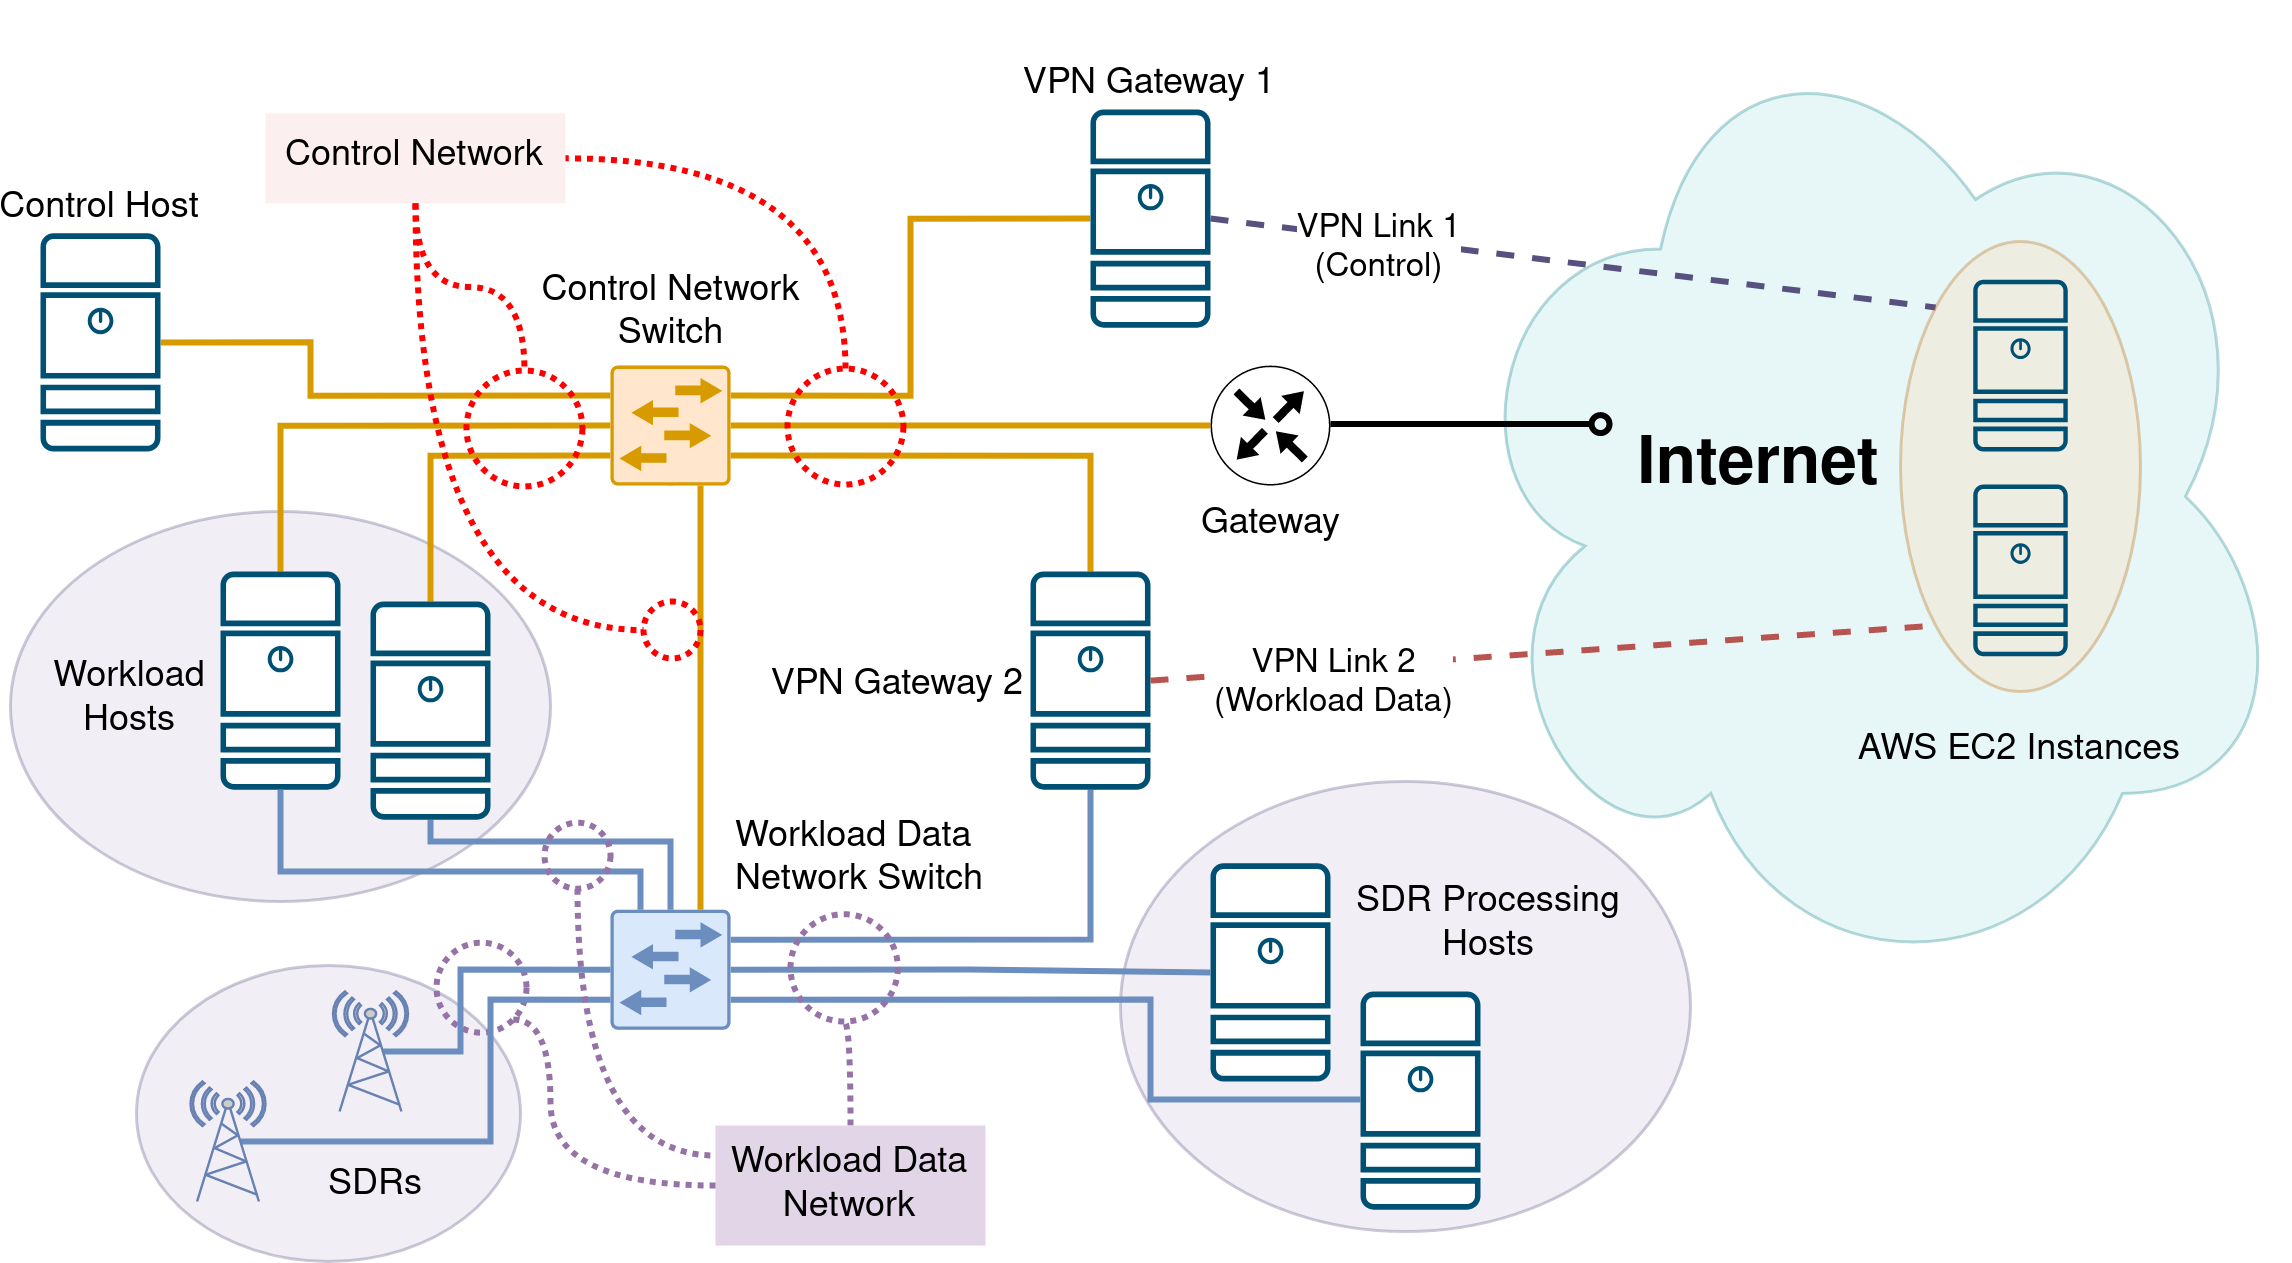
\includegraphics[width=\textwidth]{publications/2022Ainur/figures/network}
    \caption{
        Prototype architecture of \acs{EXPECA}.
        Figure originally published in \cref{paper:olguinmunoz2022ainur}.
    }\label{fig:expeca}
\end{figure}

The initial prototype architecture of \gls{EXPECA} is illustrated in \cref{fig:expeca}.
\emph{Workload hosts} act as client-side user devices.
These devices connect to either a cloudlet or cloud computing instances over the \emph{workload data network}.
Through intelligent configuration of \acsp{VLAN} and routing, traffic on this network can be forced to flow through the attached \acsp{SDR}, on of them acting as a wireless connection client and the other as an access point.
This allows us to seamlessly switch out the physical layer for experiments.
Alternatively, workload hosts can connect wirelessly via Wi-Fi to an \acs{SDR} acting as an \acs{AP}.
Finally, the \emph{control network} is used for the out-of-band configuration of testbed resources, and the \acs{VPN} links allow direct tunneled connections to cloud compute nodes on \acs{AWS}.

An implementation of this prototype was employed for the studies in \cref{paper:olguinmunoz2022cleave,paper:olguinmunoz2023realistic}.
As an initial deployment of our testbed concept, it employed
\begin{inlineenum}[itemjoin={{; }}, itemjoin*={{; and finally }}]
    \item \num{10} Raspberry Pi 4 Model B boards, acting as workload hosts
    \item two additional Raspberry Pi 4 Model boards acting as \gls{VPN} gateways as well as hosting necessary time synchronization and \gls{DNS} nameserver software
    \item a cloudlet
    \item a logging and management server
    \item a configurable number of \gls{AWS} \gls{EC2} cloud instances acting as cloud compute nodes
    \item two managed switches,
    \item two \glspl{SDR} with associated radio stack processing hosts
\end{inlineenum}.

The above prototype was formally introduced in \cref{paper:olguinmunoz2022ainur}, together with the software framework employed for its automation and experiment orchestration.
